\documentclass[a4paper, 12pt,oneside,reqno]{amsart}
\usepackage[utf8x]{inputenc}
\usepackage[T1]{fontenc}
\usepackage{tikz}
\usetikzlibrary{arrows,shapes,snakes,automata,backgrounds,petri,through,positioning}
\usetikzlibrary{intersections}
\usepackage{tikz-cd}
\usepackage{amssymb,amscd,amsthm,amsmath}
\usepackage{amsmath}
\usepackage{amssymb}
\usepackage[colorinlistoftodos]{todonotes}
\usepackage[colorlinks=true, allcolors=blue]{hyperref}

\begin{document}

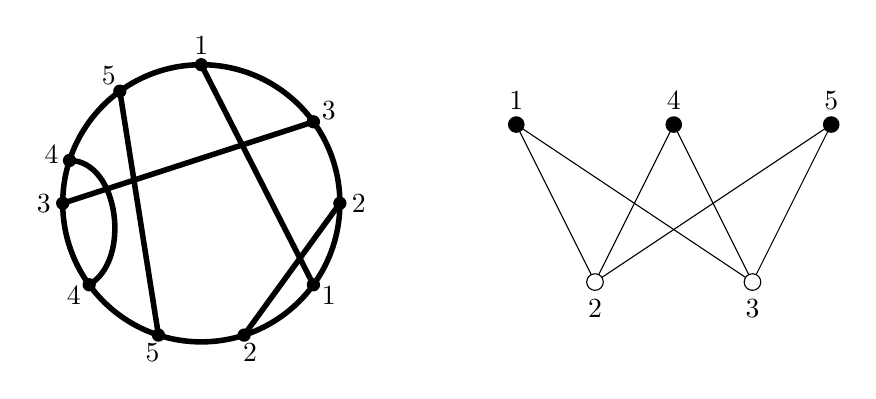
\begin{tikzpicture}
    \begin{scope}[xshift = 0cm, yshift = 0.5cm, scale =0.8,line width=2]
     \draw[line width =2] (0,0) circle (2.2);
     {\foreach \angle/ \label in
   { 90/1, 126/5, 162/4,  180/3, 216/4, 252/5, 288/2, 324/1, 0/2, 36/3}
   {
    \fill(\angle:2.5) node{$\label$};
    \fill(\angle:2.2) circle (3pt) ;
    }
}
     \draw (90:2.2) -- (324:2.2);
     \draw (126:2.2) -- (252:2.2);
     \draw (162:2.2) to [out = 0, in = 30] (216:2.2);
     \draw (180:2.2) -- (36:2.2);
     \draw (288:2.2) -- (0:2.2);
\end{scope}

\begin{scope}[xshift = 4cm, yshift = 0.5cm]
 
    \draw (0,1) -- (1,-1);
    \draw (0,1) -- (3,-1);

    \draw (2,1) -- (1,-1);
    \draw (2,1) -- (3,-1);

    \draw (4,1) -- (1,-1);
    \draw (4,1) -- (3,-1);
   
    \fill (0,1.3) node {$1$};
    \fill  (0,1) circle (3pt);

    \fill (2,1.3) node {$4$};
    \fill  (2,1) circle (3pt);

    \fill (4,1.3) node {$5$};
    \fill  (4,1) circle (3pt);

    \fill[white] (1,-1) circle (3pt);

    \fill (1,-1.1) node[below] {$2$};
    \draw  (1,-1) circle (3pt);

   \fill[white] (3,-1) circle (3pt);

   \fill (3,-1.1) node[below] {$3$};
    \draw  (3,-1) circle (3pt);
\end{scope}
      \end{tikzpicture}

\end{document}